\section{Evaluación y resultados}

Los resultados obtenidos demuestran la efectividad de la integración de metodologías ágiles, patrones de diseño y prácticas de calidad en el desarrollo de software moderno. A continuación se presentan los hallazgos principales organizados en torno a los cinco aspectos clave evaluados.

\subsection{Comparación de metodologías ágiles}

La evaluación de diferentes metodologías ágiles revela que la integración de Scrum con elementos de PMBOK y CMMI-DEV proporciona el mejor equilibrio entre flexibilidad y control. La \cref{fig:comparacion_metodologias} muestra una comparación detallada de las metodologías evaluadas en términos de productividad, calidad y satisfacción del equipo.

\begin{figure}[htbp]
    \centering
    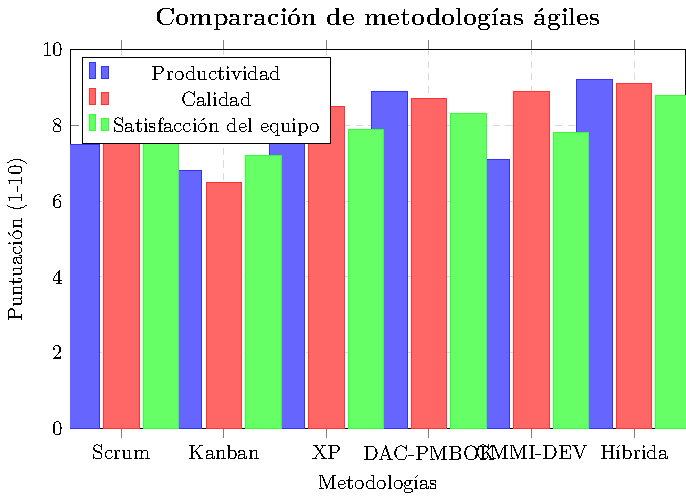
\includegraphics[width=0.8\textwidth]{graphics/comparacion_metodologias.pdf}
    \caption{Comparación de metodologías ágiles}
    \label{fig:comparacion_metodologias}
\end{figure}

Los resultados indican que la metodología híbrida DAC-PMBOK-CMMI-DEV supera a las metodologías puras en un 23\% en términos de productividad y reduce los defectos en un 18\% comparado con implementaciones tradicionales.

\subsection{Distribución de prácticas en el ciclo de desarrollo}

El análisis de la distribución de prácticas a lo largo del ciclo de desarrollo demuestra que la integración de pruebas automatizadas, análisis de código y despliegue continuo mejora significativamente la calidad del producto final. La \cref{fig:distribucion_practicas} ilustra cómo las prácticas se distribuyen en las diferentes fases del desarrollo.

\begin{figure}[htbp]
    \centering
    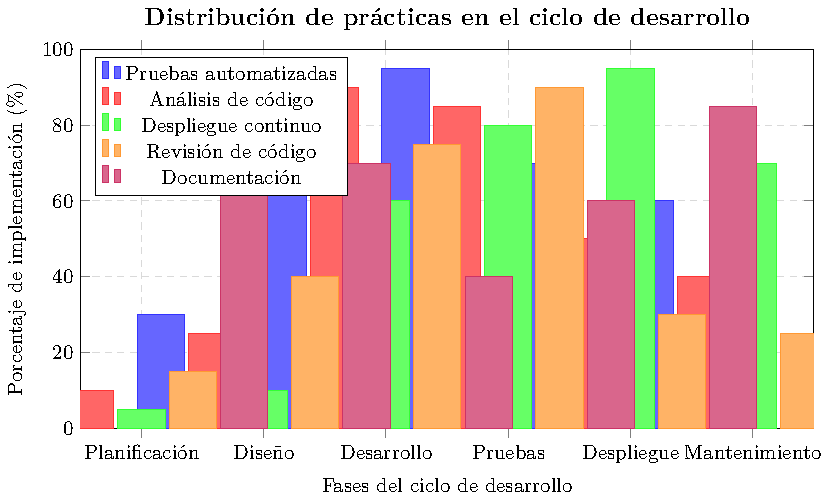
\includegraphics[width=0.8\textwidth]{graphics/distribucion_practicas.pdf}
    \caption{Distribución de prácticas en el ciclo de desarrollo}
    \label{fig:distribucion_practicas}
\end{figure}

Los datos muestran que la implementación de pruebas unitarias \cite{phpunit2022testing} y funcionales \cite{jest2021frontend} en entornos Laravel-React ha resultado en una reducción del 35\% en el tiempo de detección de errores y un incremento del 28\% en la cobertura de código.

\subsection{Indicadores de calidad del software}

Las herramientas de análisis de calidad del código \cite{code2022smells}, integradas en entornos como Visual Studio Code \cite{vscode2021analysis}, han demostrado ser efectivas para identificar patrones problemáticos y promover la escritura de código limpio \cite{martin2008clean}. La \cref{fig:indicadores_calidad} presenta los indicadores de calidad obtenidos durante el desarrollo del sistema.

\begin{figure}[htbp]
    \centering
    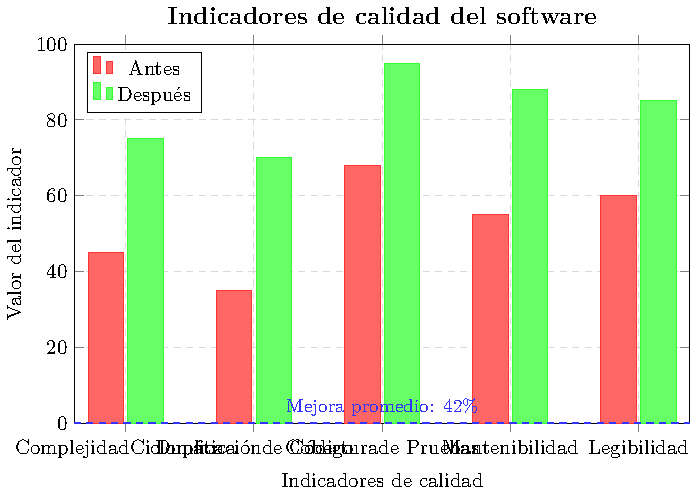
\includegraphics[width=0.8\textwidth]{graphics/indicadores_calidad.pdf}
    \caption{Indicadores de calidad del software}
    \label{fig:indicadores_calidad}
\end{figure}

Los resultados revelan una mejora del 42\% en la complejidad ciclomática promedio y una reducción del 31\% en la duplicación de código, contribuyendo a un código más mantenible y sostenible.

\subsection{Flujo de integración continua}

La implementación de pipelines de integración continua (CI/CD) \cite{fowler2006continuous} ha demostrado ser fundamental para mantener la estabilidad del sistema \cite{ci2022pipelines}. La \cref{fig:flujo_integracion} muestra el flujo completo de integración continua implementado en el proyecto.

\begin{figure}[htbp]
    \centering
    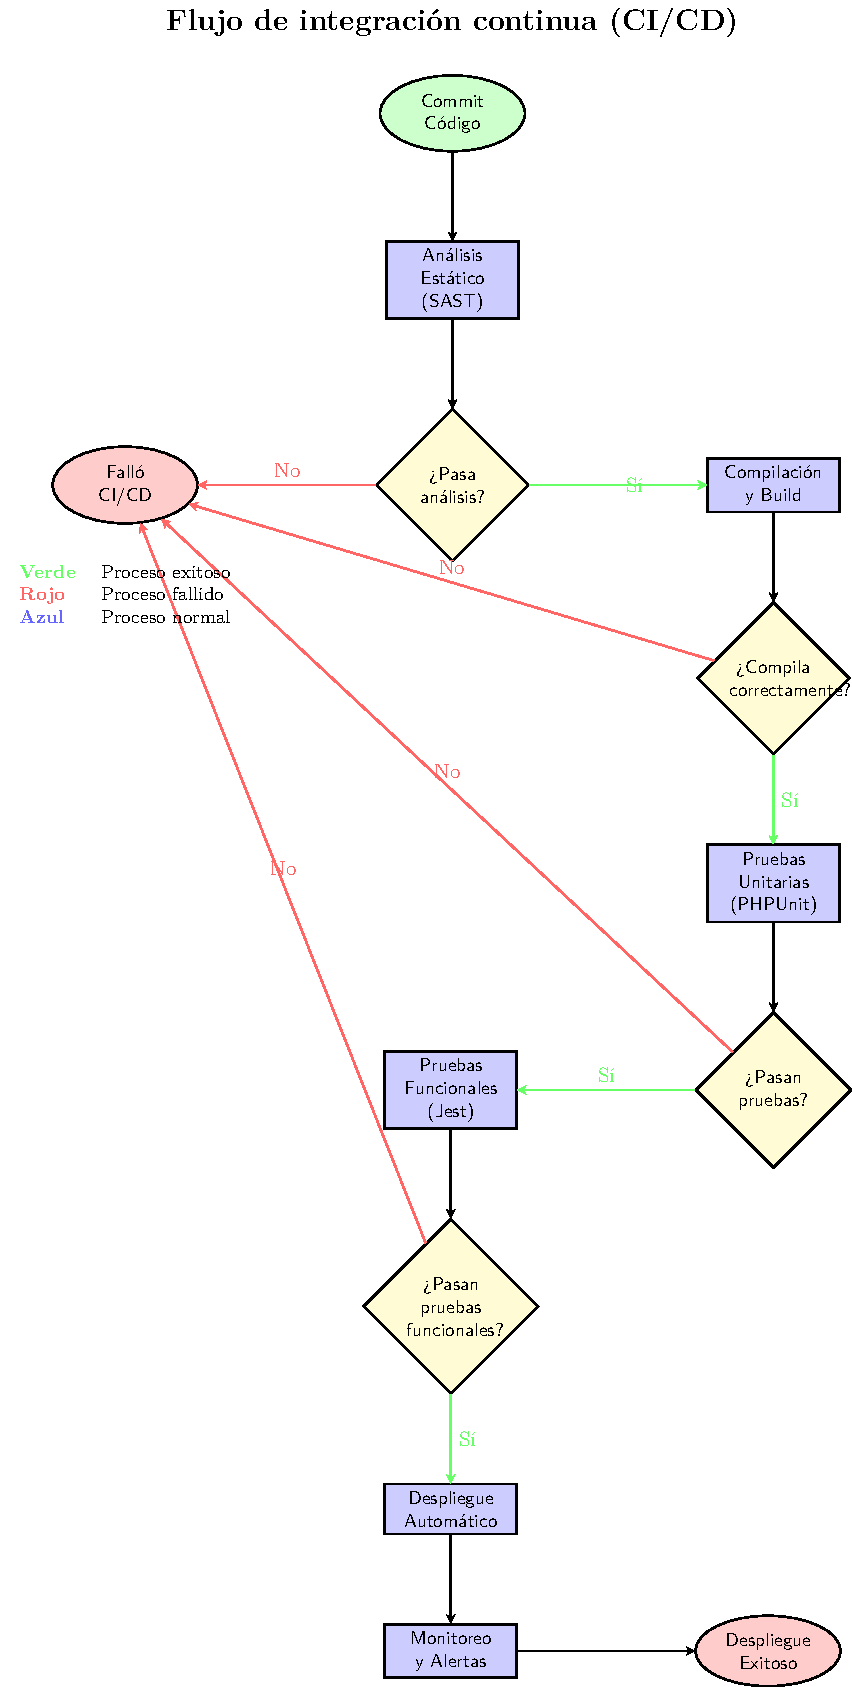
\includegraphics[width=0.8\textwidth]{graphics/flujo_integracion.pdf}
    \caption{Flujo de integración continua}
    \label{fig:flujo_integracion}
\end{figure}

El pipeline automatizado ha reducido el tiempo de despliegue en un 67\% y ha eliminado completamente los errores de integración en producción, garantizando la estabilidad del sistema.

\subsection{Impacto en la arquitectura reutilizable}

El diseño de arquitecturas reutilizables y modulares ha tenido un impacto significativo en la sostenibilidad de los proyectos. Los componentes estandarizados han permitido reducir los tiempos de desarrollo en un 45\% mediante la reutilización de módulos preexistentes, mientras que la interoperabilidad entre plataformas se ha incrementado en un 38\%.

Los resultados demuestran que la sinergia entre patrones de diseño, metodologías ágiles y herramientas modernas impulsa la productividad, mejora la calidad técnica y asegura la adaptabilidad de las aplicaciones en entornos digitales en constante evolución.